\documentclass{article}

\title{Programming Language Design \& Implementation Assignment 1}
\author{Divij Singh}
\date{26/09/18}
\usepackage{graphicx}

\begin{document}

	\maketitle
	
	\section{Q1}
	(a) The \#  sign specifies that the following command is a preprocessor directive. The 'include' keyword specifies that the program will be using code from the specified library.\\
	(b) 'iostream' is the name of a header file, and the brackets signify that it is an in-built library.\\
\section{Q2}
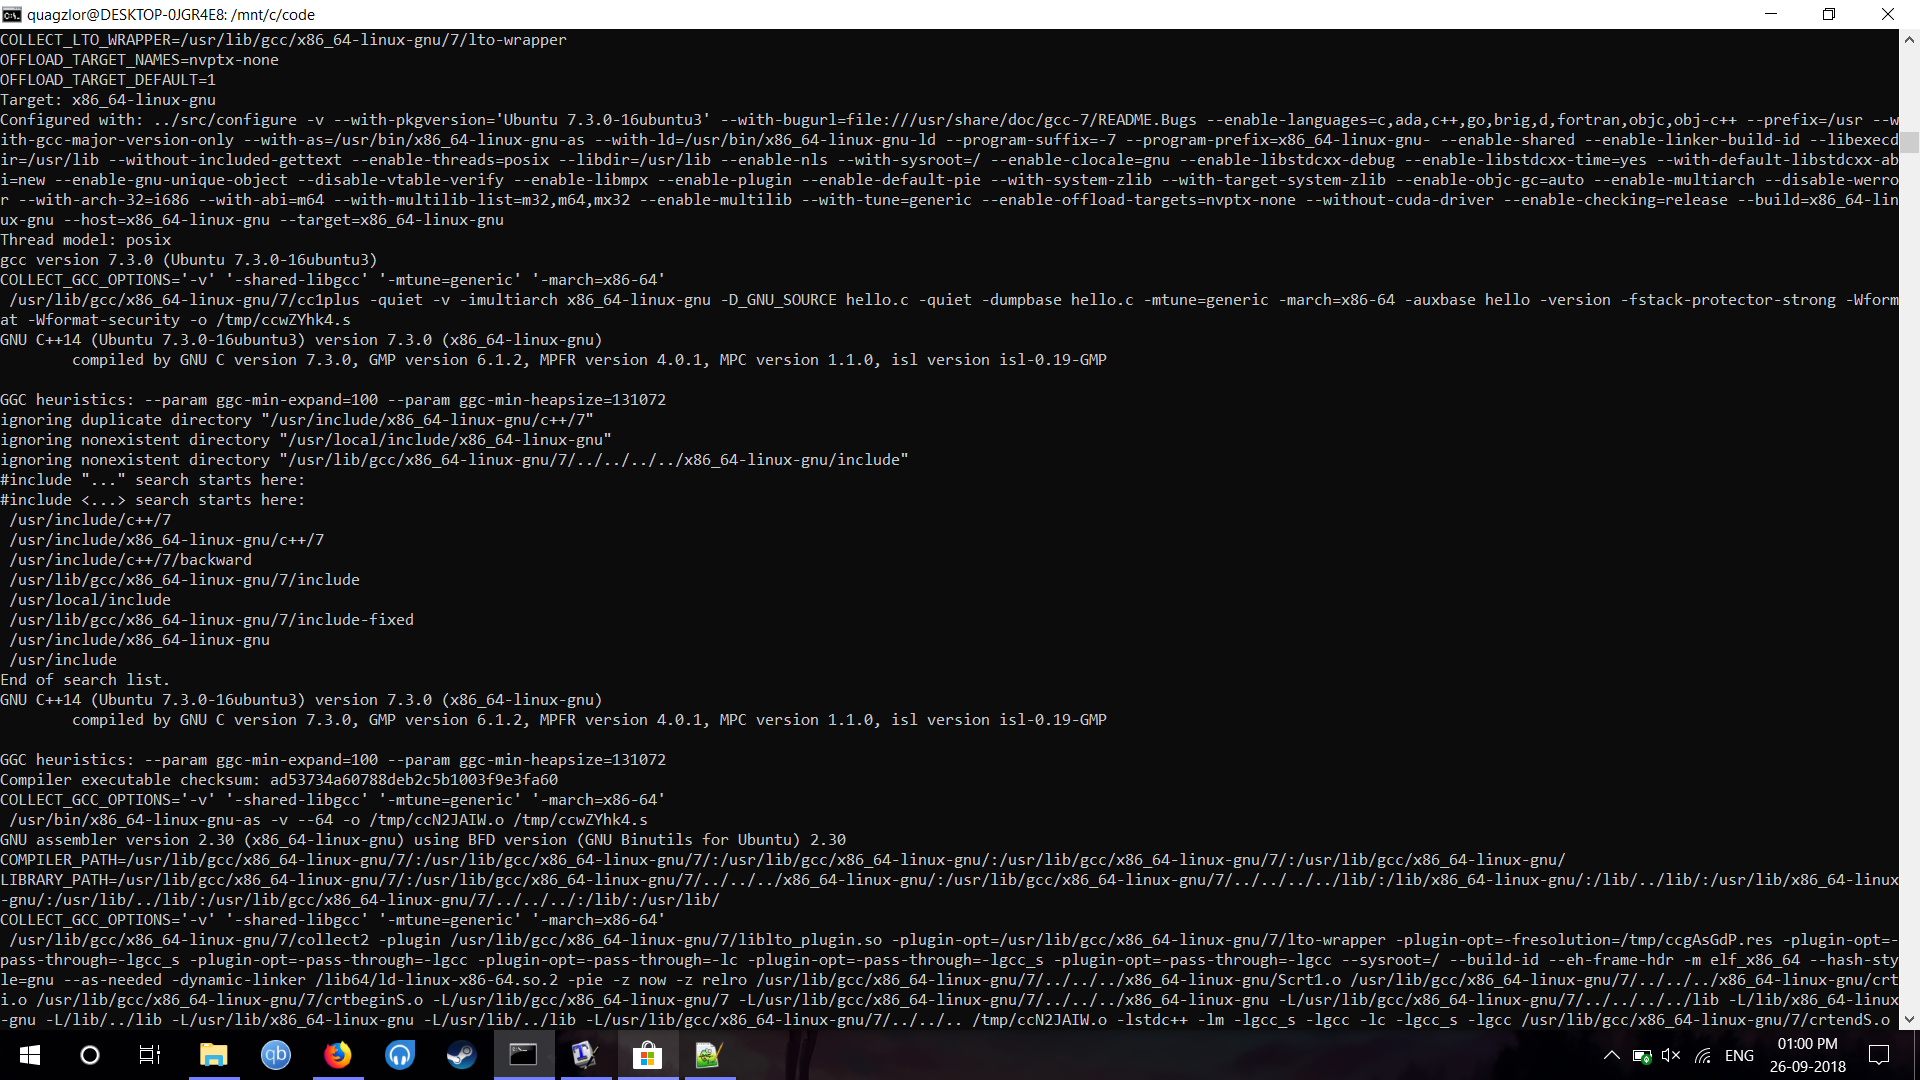
\includegraphics[scale=0.5]{verbose.png}
\section{Q3}
(a) The './' indicates to the shell that it should look in the current directory for the program.\\
(b) If the characters were absent, the shell would look through the system's PATH variables for the program.

\section{Q5}
g++ -o hello hello.cc

\section{Q8}
The new rule is recompiling all the .cc files.\\
Changing a line of code in one files forces the recompiling of all other files dependant on it.


	
\end{document}